\documentclass[ucs,10pt]{beamer}
 
% Template for talks using the Logo of STCE and Corporate Design of RWTH Aachen
% adapted from:
% https://www.mi.fu-berlin.de/w/Mi/BeamerTemplateCorporateDesign

\usepackage{amsmath,dsfont,listings}

%%% STCE logo
% small version for upper right corner of normal pages
\pgfdeclareimage[height=0.9cm]{university-logo}{rwth_i12_softw-werkz_en_rgb.png}
\logo{\pgfuseimage{university-logo}}
% large version for upper right corner of title page
\pgfdeclareimage[height=1cm]{big-university-logo}{rwth_i12_softw-werkz_en_rgb.png}
\newcommand{\titleimage}[1]{\pgfdeclareimage[height=2cm]{title-image}{#1}}
\titlegraphic{\pgfuseimage{title-image}}
%%% end STCE logo

% NOTE: 1cm = 0.393 in = 28.346 pt;    1 pt = 1/72 in = 0.0352 cm
\setbeamersize{text margin right=3.5mm, text margin left=7.5mm}  % text margin

% colors to be used
\definecolor{text-grey}{RGB}{51, 51, 51} % grey text on white background
\definecolor{bg-grey}{rgb}{0.66, 0.65, 0.60} % grey background (for white text)
\definecolor{rwth-blue}{RGB}{0, 83, 159} % blue text
\definecolor{rwth-green}{RGB}{153, 204, 0} % green text
\definecolor{rwth-red}{RGB}{204, 0, 0} % red text (used by \alert)

% switch off the sidebars
% TODO: loading \useoutertheme{sidebar} (which is maybe wanted) also inserts
%   a sidebar on title page (unwanted), also indents the page title (unwanted?),
%   and duplicates the navigation symbols (unwanted)
\setbeamersize{sidebar width left=0cm, sidebar width right=0mm}
\setbeamertemplate{sidebar right}{}
\setbeamertemplate{sidebar left}{}
%    XOR
% \useoutertheme{sidebar}

% frame title
% is truncated before logo and splits on two lines
% if neccessary (or manually using \\)
\setbeamertemplate{frametitle}{%
    \vskip-30pt \color{purple}\large%
    \begin{minipage}[b][23pt]{80.5mm}%
    \flushleft\insertframetitle%
    \end{minipage}%
}

%%% title page
% TODO: get rid of the navigation symbols on the title page.
%   actually, \frame[plain] *should* remove them...
\setbeamertemplate{title page}{
% upper right: STCE logo
\vskip2pt\hfill\pgfuseimage{big-university-logo} \\
\vskip6pt\hskip3pt
% title image of the presentation
% set the title and the author
\begin{center}
\vskip4pt
\large \inserttitle \vskip5pt  \small \insertsubtitle
\vskip8pt
	\normalsize \insertauthor %\\ 
	%\includegraphics[width=2cm]{../../foto_naumann}	
\\ [5mm]
	\footnotesize \insertinstitute 
\end{center}
}
%%% end title page

%%% colors
\usecolortheme{lily}
\setbeamercolor*{normal text}{fg=black,bg=white}
\setbeamercolor*{alerted text}{fg=rwth-red}
\setbeamercolor*{example text}{fg=rwth-green}
\setbeamercolor*{structure}{fg=rwth-blue}

\setbeamercolor*{block title}{fg=white,bg=black!50}
\setbeamercolor*{block title alerted}{fg=white,bg=black!50}
\setbeamercolor*{block title example}{fg=white,bg=black!50}

\setbeamercolor*{block body}{bg=black!10}
\setbeamercolor*{block body alerted}{bg=black!10}
\setbeamercolor*{block body example}{bg=black!10}

\setbeamercolor{bibliography entry author}{fg=rwth-blue}
% TODO: this doesn't work at all:
\setbeamercolor{bibliography entry journal}{fg=text-grey}

\setbeamercolor{item}{fg=rwth-blue}
\setbeamercolor{navigation symbols}{fg=text-grey,bg=bg-grey}
%%% end colors

%%% headline
\setbeamertemplate{headline}{
\vskip4pt\hfill\insertlogo\hspace{3.5mm} % logo on the right

\vskip6pt\color{rwth-blue}\rule{\textwidth}{0.4pt} % horizontal line
}
%%% end headline

%%% footline
\newcommand{\footlinetext}{\insertshortinstitute, \insertshorttitle}
\setbeamertemplate{footline}{
\vskip5pt\color{rwth-blue}\rule{\textwidth}{0.4pt}\\ % horizontal line
\vskip2pt
\makebox[123mm]{\hspace{7.5mm}
\color{rwth-blue}\footlinetext
\hfill \raisebox{-1pt}{\usebeamertemplate***{navigation symbols}}
\hfill \insertframenumber}
\vskip4pt
}
%%% end footline

%%% settings for listings package
\lstset{extendedchars=true, showstringspaces=false, basicstyle=\footnotesize\sffamily, tabsize=2, breaklines=true, breakindent=10pt, frame=l, columns=fullflexible}
\lstset{language=C++} % this sets the syntax highlighting
\lstset{mathescape=true} % this switches on $...$ substitution in code
% enables UTF-8 in source code:
\lstset{literate={ä}{{\"a}}1 {ö}{{\"o}}1 {ü}{{\"u}}1 {Ä}{{\"A}}1 {Ö}{{\"O}}1 {Ü}{{\"U}}1 {ß}{\ss}1}
%%% end listings
  

\begin{document}
\title[{\tt info@stce.rwth-aachen.de}]{\textcolor{rwth-blue}{Software Lab Computational Engineering Science} \vspace{.2cm} \\ {\small Group 12, Pusher Mechanism}}
\author[Group 12)]{Aaron Floerke, Arseniy Kholod, Xinyang Song and Yanliang Zhu} 
\institute[Software Lab CES]{
{Informatik 12: Software and Tools for Computational Engineering (STCE)} \\ RWTH Aachen University \vspace{.5cm}
}
\date[]{24.06.2024}



\begin{frame}[plain]
\titlepage
\end{frame}

\begin{frame}
	\frametitle{Contents}
\tableofcontents
\end{frame}



\section{Visualization}

\begin{frame}
\frametitle{Visualization \\
    \small \color{rwth-blue} The Four-Bar/Pusher Mechanism}
    \begin{itemize}
        \item Online Demo: \url{https://www.geogebra.org/m/BueCG9ch}
    \end{itemize}
    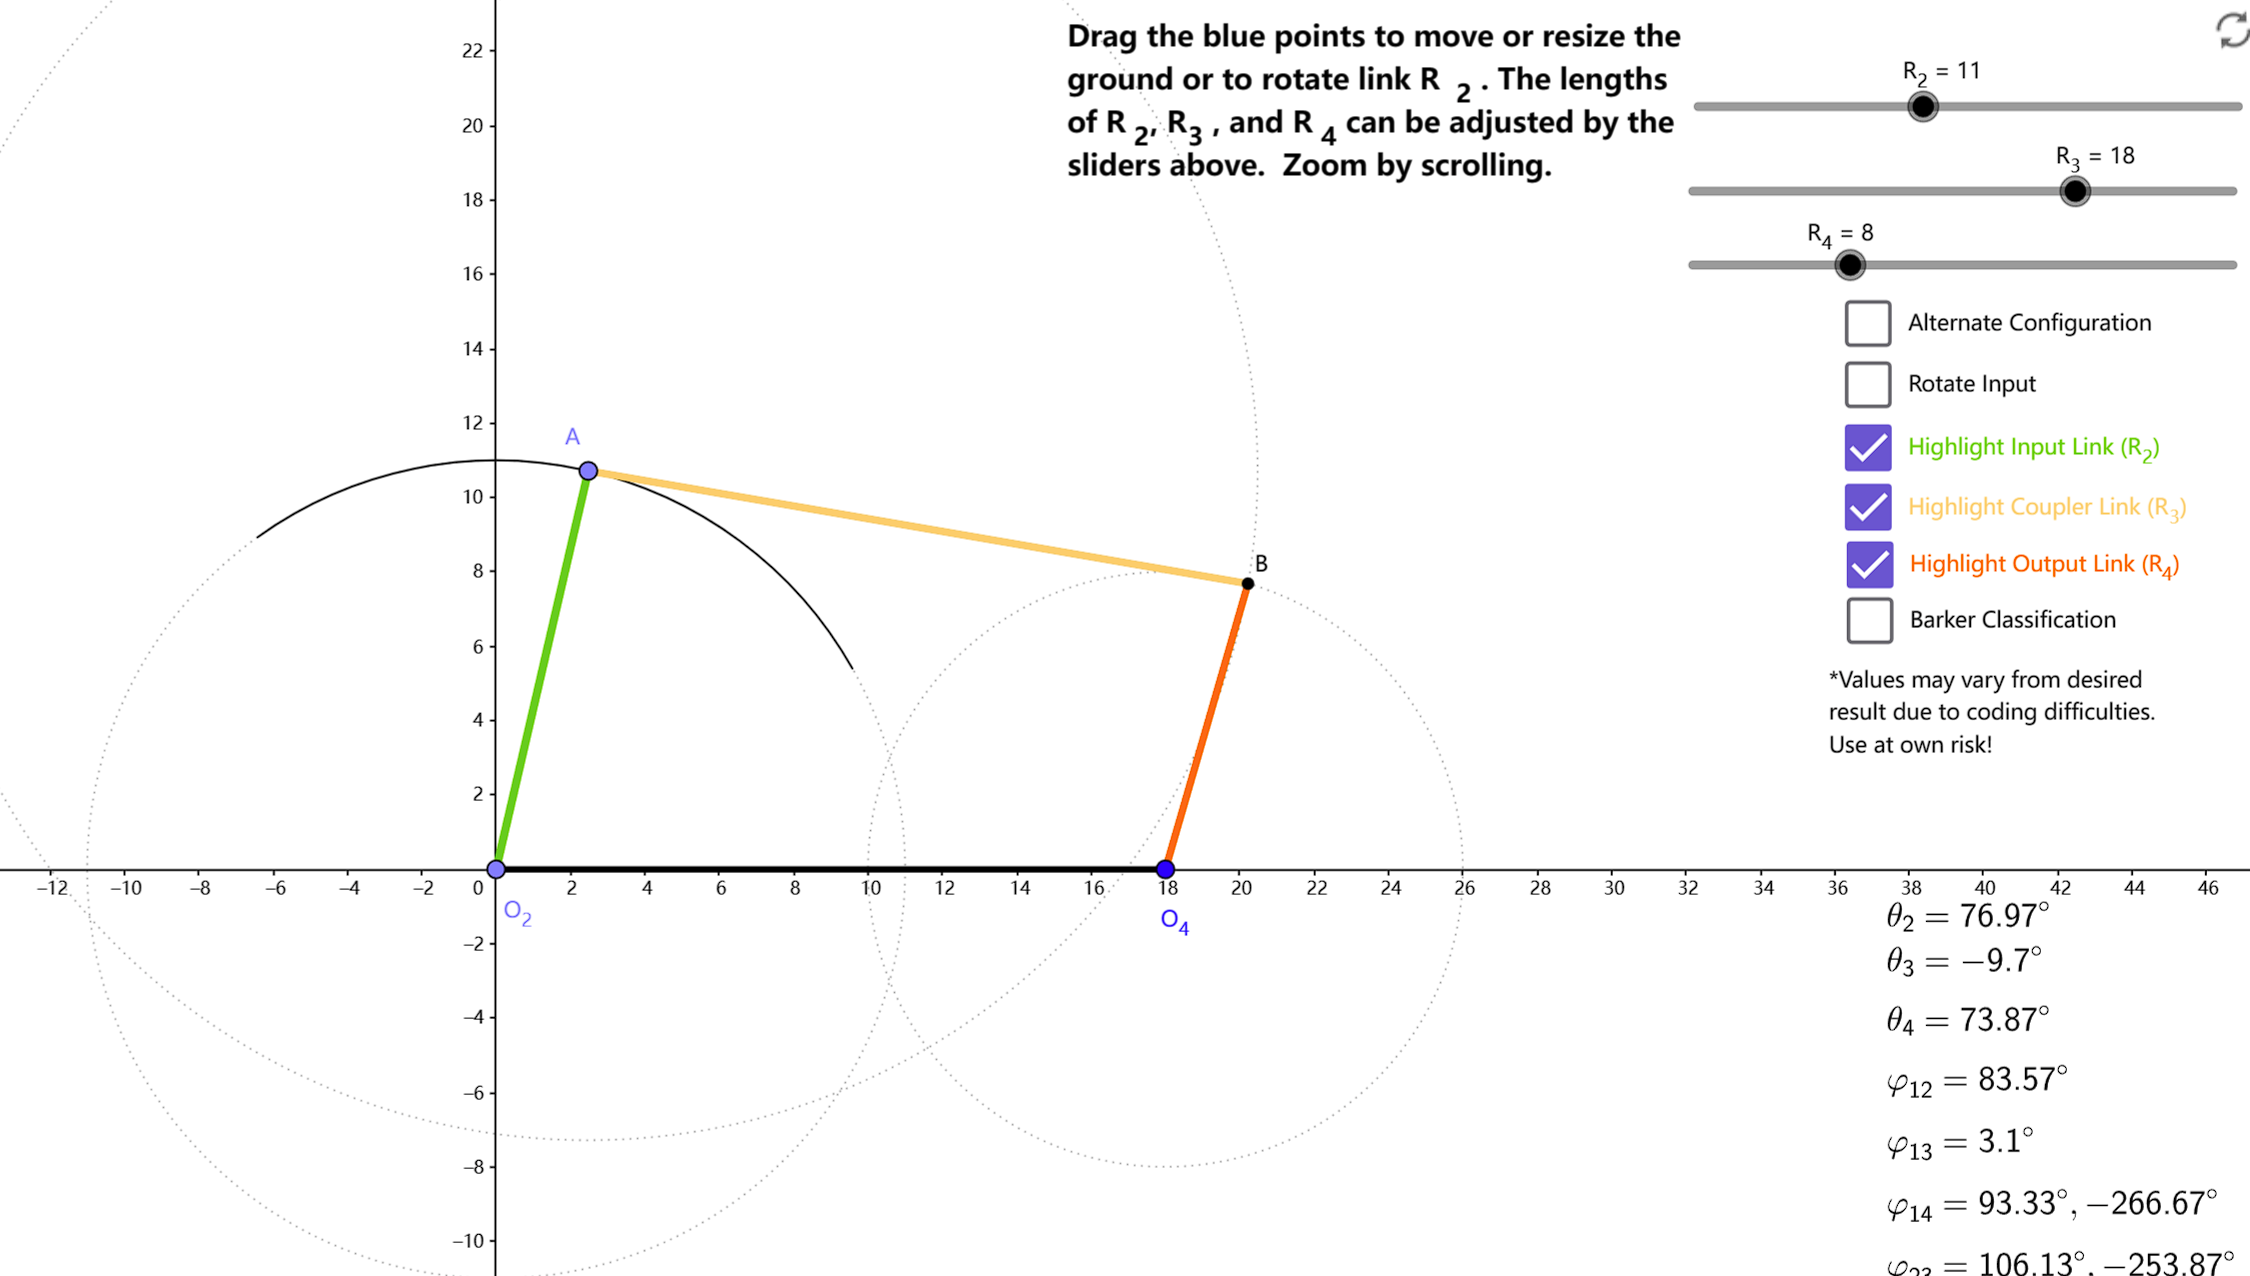
\includegraphics[width=0.9\linewidth]{./Used_Picture/Online_Demo_1.png}
\end{frame}



\section{User Requirements}


\begin{frame}
\frametitle{User Requirements}
    \begin{itemize}
        \item Simulate the motion of the pusher mechanism.
        \item Implement all motion types for the four-bar linkage with one bar fixed (8 cases according to \url{https://en.wikipedia.org/wiki/Four-bar_linkage}).
        \item Implement GUI with motion animation and the ability to choose geometrical parameters.
        \item Solve an optimization problem.
    \end{itemize}
\end{frame}


\begin{frame}
\frametitle{User Requirements \\
	\small \color{rwth-blue} Optimization problem}
        \begin{center}
            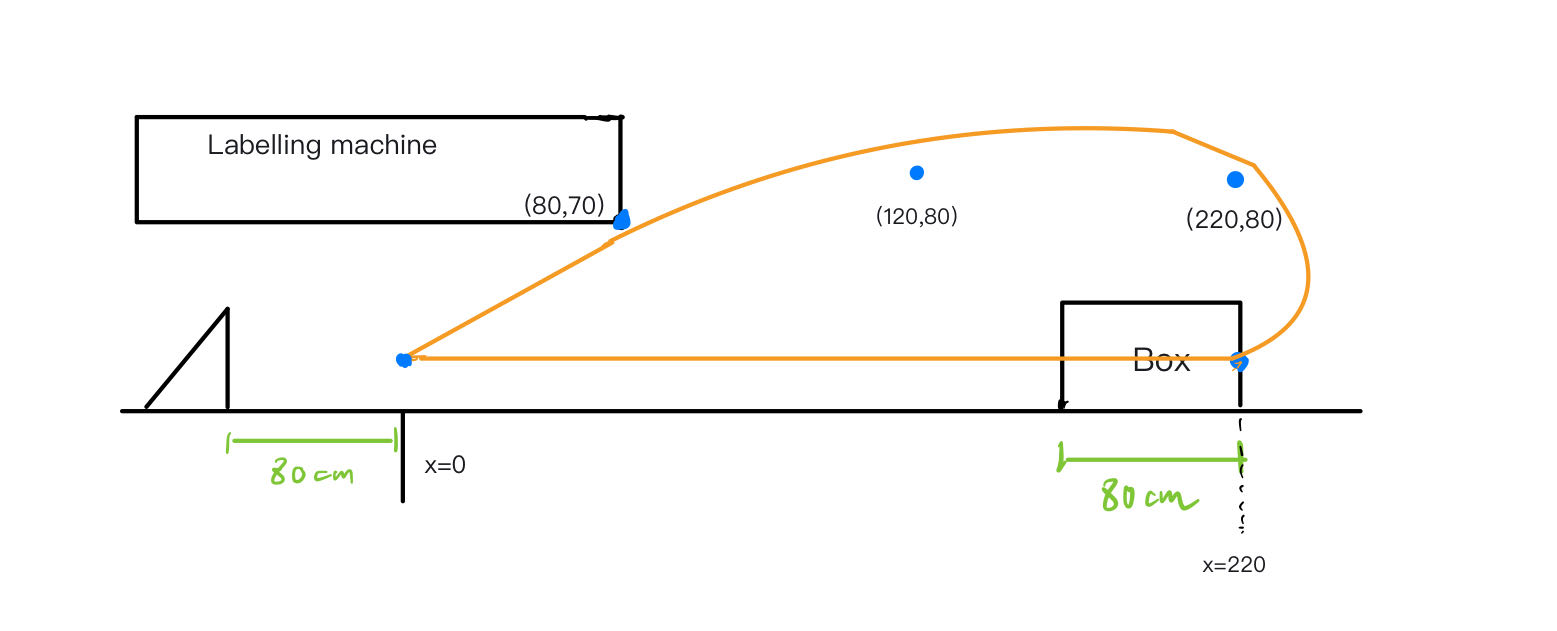
\includegraphics[width=0.75\linewidth]{./Used_Picture/Example_1.jpg}
        \end{center}
	\begin{itemize}
        \item Find suitable parameters for the pusher mechanism to meet requirements:
            \begin{itemize}
                \item Push box with size $80\times60$ from $x=220$ to $x=0$
                \item Do not cross the area of the labelling machine (Area with $x<80$ and $y>70$).
                \item Pass above points $(120, 80)$ and $(220, 80)$
            \end{itemize}
        \item Provide the following data for the designed four-bar mechanism:
            \begin{itemize}
                \item Position of the two fixed pivot positions
                \item Lengths of the three moving links and of the fourth base link
                \item The position of the couple offset point relative to the coupler
            \end{itemize}
	\end{itemize}
        {\small *all coordinates and length are in cm}
\end{frame}



\section{System Requirements}

\begin{frame}
\frametitle{System Requirements \\
    \small \color{rwth-blue} Functional}
    \begin{itemize}
        \item \textbf{Four-bar linkage model}:
        \begin{itemize}
            \item System simulates the motion of the four-bar linkage.
            \item System distinguishes between all different motion cases.
            \item System does not crash with any input of geometrical configuration.
            \item System provides asserts or/and exception mechanisms to validate input data.
        \end{itemize}
        \item \textbf{Tests}:
        \begin{itemize}
            \item Implement test cases to cover all motion cases.
            \item Provide reference data to compare results with.
            \item Implement test cases with bad input to test system stability.
        \end{itemize}
    \end{itemize}
\end{frame}


\begin{frame}
\frametitle{System Requirements \\
    \small \color{rwth-blue} Functional}
    \begin{itemize}
        \item \textbf{Graphical User Interface}:
        \begin{itemize}
            \item GUI provides the four-bar linkage visualization.
            \item User can input geometrical data by moving a point on a slide bar or/and using a keyboard.
            \item GUI reacts to new input data by changing the four-bar linkage visualization accordingly.
            \item GUI provides animation of the four-bar linkage motion.
            \item User can choose parameters of this motion, e.g. restrict rotation angles.
            \item User can move linkage by pulling an input bar using a computer mouse.
            \item GUI is coupled with the four-bar linkage model to use implemented motion cases for animation. 
        \end{itemize}
        \item \textbf{Optimization problem}:
        \begin{itemize}
            \item It should be possible to find a solution (manually) for the optimization problem using the four-bar linkage model.
            \item GUI visualizes the solution.
        \end{itemize}
    \end{itemize}
\end{frame}

\begin{frame}
\frametitle{System Requirements \\
    \small \color{rwth-blue} Non-Functional}
    \begin{itemize}
        \item \textbf{Performance}:
        \begin{itemize}
            \item The four-bar linkage model is fast enough to provide smooth GUI animations.
            \item GUI animations are not slower than 30 frames per second.
        \end{itemize}
        \item \textbf{Usability}:
        \begin{itemize}
            \item Every essential part of the four-bar linkage model is well documented.
            \item GUI is easy to operate.
            \item GUI functionalities are well documented.
            \item All changeable parameters are explained.
            \item GUI animation displays trajectories of bar connection points.
        \end{itemize}
        \item \textbf{Locality}:
        \begin{itemize}
            \item GUI and the four-bar linkage model both can run on a local machine.
            \item Additionally: Local GUI should be able to connect to a remote four-bar linkage model.
            \item Additionally: It should be possible to provide a web GUI.
        \end{itemize}
    \end{itemize}
\end{frame}

\section{Prototype}

\begin{frame}
\frametitle{Prototype \\
    \small \color{rwth-blue} Sequence diagram for animation}
    \begin{center}
        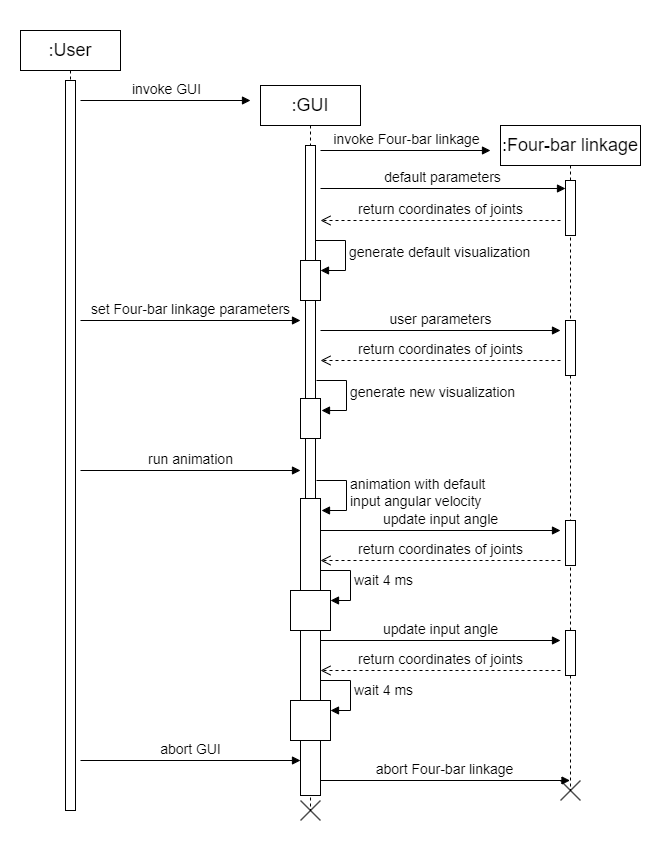
\includegraphics[width=0.5\linewidth]{Used_Picture/sequence_diagramm_animation.png}
    \end{center}
\end{frame}

\begin{frame}
\frametitle{Prototype \\
    \small \color{rwth-blue} GUI}

\end{frame}


\section{Project Management}

\begin{frame}
\frametitle{Project Management \\
    \small \color{rwth-blue} Gantt Chart}
\end{frame}


\section{Summary and Conclusion}

\begin{frame}
\frametitle{Summary and Conclusion}
    \begin{itemize}
        \item \textbf{User requirements}
        \item \textbf{Optimization problem}
        \item \textbf{System requirements}
        \item \textbf{Prototype}:
        \begin{itemize}
            \item Sequence diagram for communication between user, GUI, and Four-bar linkage model.
            \item Graphical user interface visualization.
        \end{itemize}
        \item \textbf{Project  with Gantt Chart}
        \item \textbf{Next tasks}:
        \begin{itemize}
            \item Design classes, interfaces, functions.
            \item Design detailed use-cases.
            \item Choose languages and environment to implement Four-bar linkage model and GUI.
            \item Implementation and documentation.
            \item Implement tests and use-cases.
            \item Solve the optimization problem.
        \end{itemize}
    \end{itemize}
\end{frame}

\end{document}
